\documentclass[twocolumn, a4paper]{article}
\usepackage[a4paper, left = 1.75cm, right = 1.75cm, top = 1.75cm, bottom = 1.75cm]{geometry}
\usepackage[style = numeric, sorting = none]{biblatex}
\usepackage{pgfplots}
\usepackage[T1]{fontenc}
\usepackage{graphicx}
\usepackage{arydshln}
\usepackage[UKenglish]{babel}
\usepackage[UKenglish]{isodate}

\graphicspath{{./images/}}
\addbibresource{refs.bib}

\cleanlookdateon

\renewcommand*{\bibfont}{\footnotesize}

\author{
  George Herbert\\
  \texttt{cj19328@bristol.ac.uk}
}

\title{\vspace{-2em}Parallelising d2q9-bgk.c with MPI}

\begin{document}

\maketitle

\begin{abstract}
  \texttt{d2q9-bgk.c} implements the Lattice Boltzmann method (LBM) to simulate a fluid density on a lattice.
  This report analyses the techniques I utilised to parallelise \texttt{d2q9-bgk.c} with MPI, and port \texttt{d2q9-bgk.c} to a GPU with OpenCL.
\end{abstract}

\section{Single Program, Multiple Data}

\subsection{Hypothesis}

I previously achieved a substantial performance improvement producing a multithreaded implementation of \texttt{d2q9-bgk.c} with OpenMP.
However, since OpenMP was built for shared-memory parallelism, my implementation could not utilise more than one node of BC4, which was a considerable restriction.

Single program, multiple data (SPMD) is a form of parallelism in which independent processes run the same program.
Message Passing Interface (MPI) is a specification for a library interface for passing messages between processes.
Therefore, I hypothessied that an implementation of \texttt{d2q9-bgk.c} with distributed memory parallelism that ran on multiple processes across multiple nodes---with MPI being used for interprocess communication---would provide an even more substantial performance improvement.

\subsection{Compiler}

I used the \texttt{mpiicc} wrapper script, which compiled my program with the Intel C Compiler Classic (version 19.1.3.304) and set up the include and library paths for the Intel MPI library.

\subsection{Load Balancing}

I had to explicitly assign different sections of the grid to different processes.
It was crucial for the distribution to be adequately balanced to minimise the amount of time processes' spent blocked.

Since the \texttt{cells} grid was stored in row-major order, I split the grid horizontally between processes to take advantage of memory locality.
I created a procedure \texttt{allocate\_rows} to balance the load; the procedure assigned each process at least $\lfloor\frac{y}{n}\rfloor$ consecutive rows, with the first $y - \lfloor\frac{y}{n}\rfloor n$ processes each assigned an additional consecutive row, where $y$ was the number of rows and $n$ the number of processes.
Additionally, since updating the value of a given cell required the values of all adjacent cells, each process contained two additional rows reserved for cells in the top and bottom rows of the preceding and succeeding ranks, respectively.
Figure \ref{fig:rows} displays an example allocation for a grid with five rows, split between two processes; the rows allocated to a specific process are highlighted in green, with additional rows required to correctly updated the edge rows highlighted in red.

\begin{figure}[htbp]
  \centering
  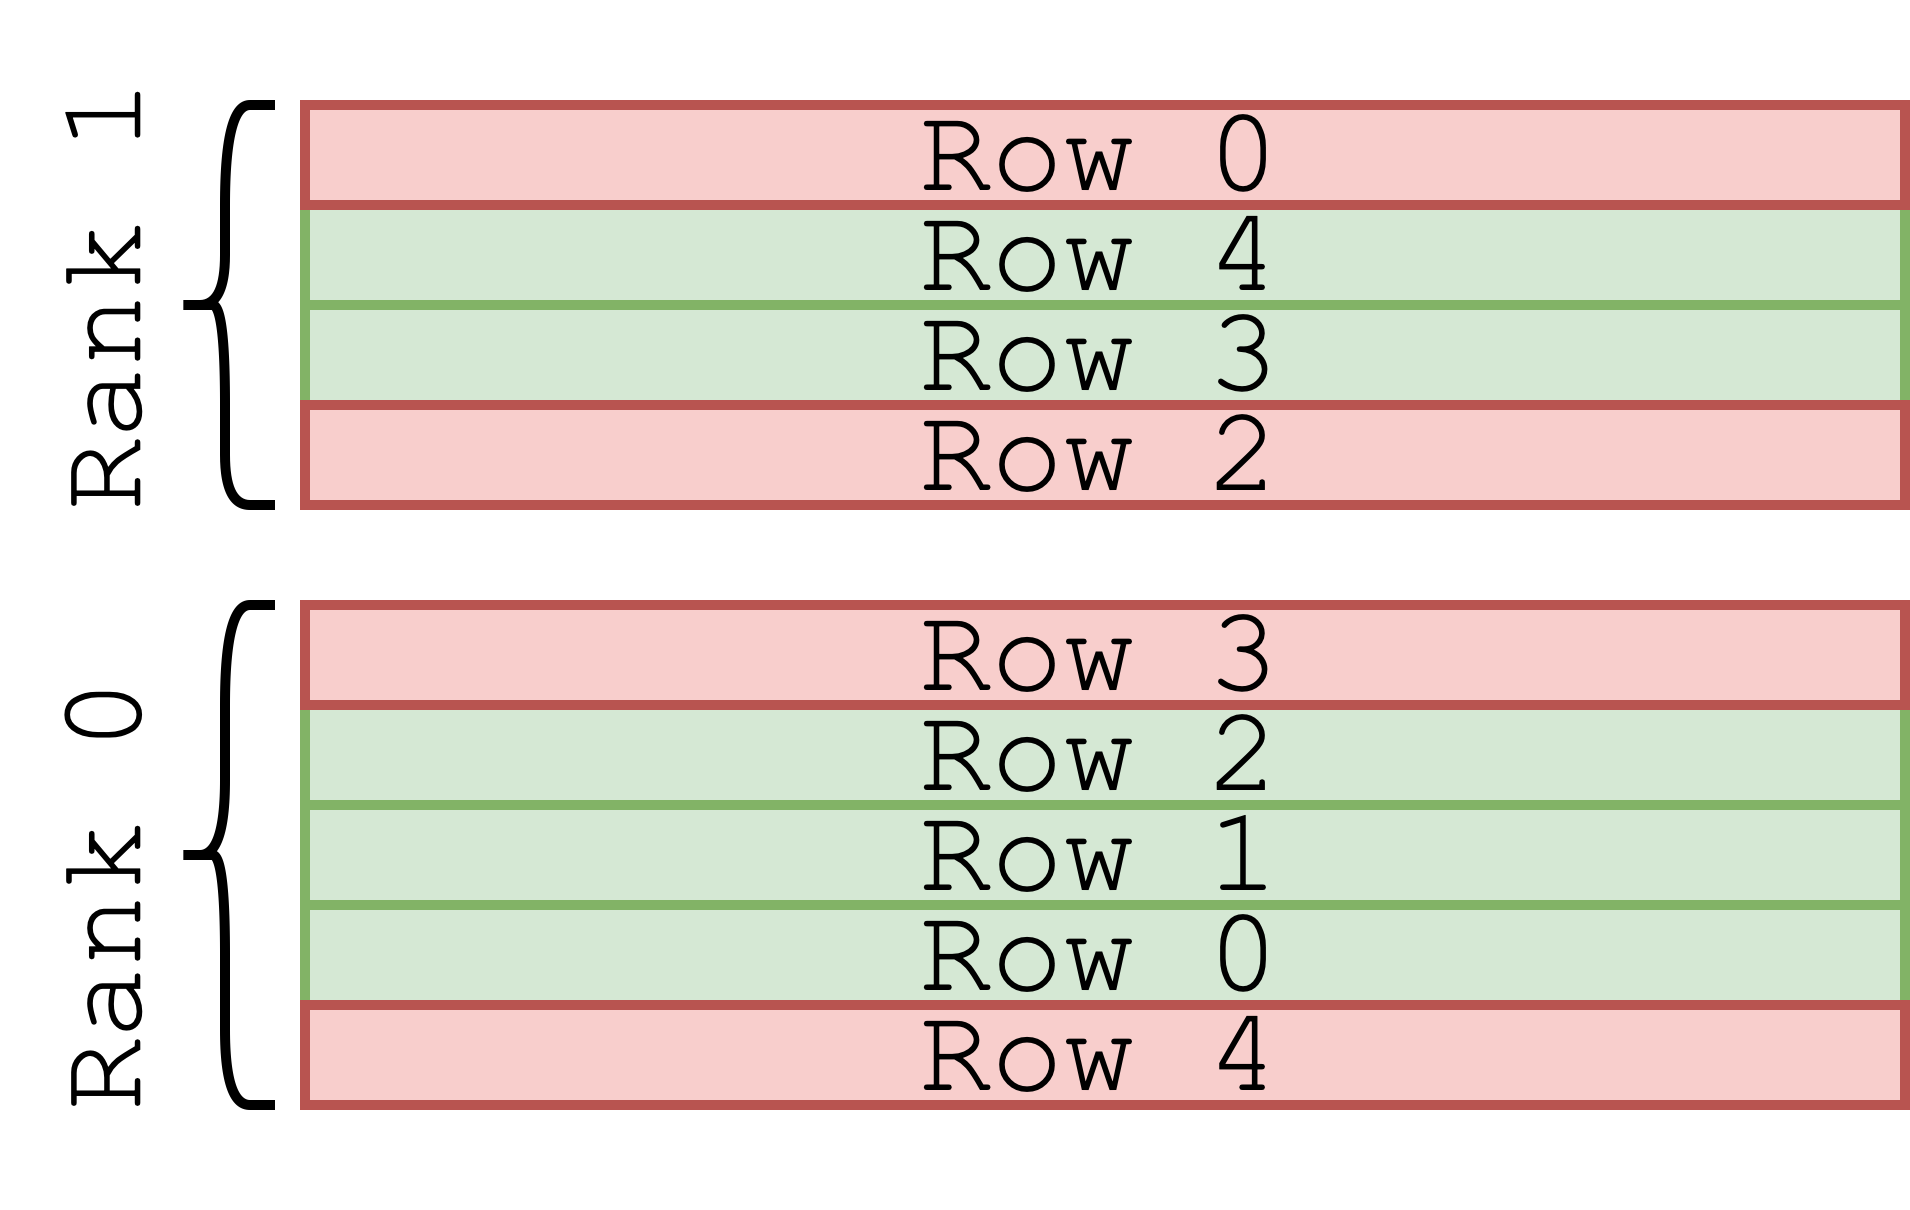
\includegraphics[width=.75\linewidth]{rows.png}
  \caption{Row allocation example with five rows and two processes}\label{fig:rows}
\end{figure}

I decided against splitting on a sub-row level to avoid unnecessarily increasing the complexity of my program and incurring an additional computational overhead.

\subsection{Halo Exchange}

Since processes are assigned their own virtual memory region, I had to explicitly send the contents of edge rows to neighbouring ranks at the conclusion of each timestep.
To do so, I created a \texttt{halo\_exchange} procedure.
The procedure copied the bottom-most row allocated to each process into the \texttt{send\_row\_buffer} array.
I used the \texttt{MPI\_Sendrecv} procedure to send this buffer to the \texttt{receive\_row\_buffer} of the preceding rank.
The values in the \texttt{receive\_row\_buffer} were then copied into the top additional row.
The same process was then repeated for the top-most row, which was sent to the succeeding rank.

\subsection{Collating}

I created a \texttt{collate} procedure to be executed once all iterations of the \texttt{timestep} procedure were complete.
The procedure had two purposes.
The first purpose was to transfer the the final state of the cells allocated to each process to the master process (i.e. rank zero).
The second purpose was to transfer the partial average velocity values to the master process, and use these values to calculate the correct average velocity at each timestep.

I used the \texttt{MPI\_Send} procedure to send the final state of the cells allocated to each process to the master process.
The master process received these values by executing the \texttt{MPI\_Recv} procedure once for each process.

I also used the \texttt{MPI\_Send} procedure to send the partial average velocity values held by each process to the master process.
The master process received these arrays of values consecutively from each process using the \texttt{MPI\_Recv} procedure, and summed them into a global average velocities array.
Once the arrays had been summed, the \texttt{colate} procedure multiplied each element by \texttt{params.num\_non\_obstacles\_r} in the master process to calculate the correct average velocity at each timestep.

\subsection{Results}

Table \ref{tab:mpi} displays the results of my MPI implementation.
Each time was an average of three runs on BlueCrystal Phase 4 (BC4) compute nodes; which were each a Lenovo nx360 M5, which contained two 14-core 2.4 GHz Intel E5-2680 v4 (Broadwell) CPUs and 128 GiB of RAM \cite{bcp4}.
My MPI implementation provided a substantial speedup over both my serial optimised implementation, as well as my OpenMP implementation.
The speedup was primarily achieved by executing sections of the \texttt{timestep} procedure in parallel, and utilising 112 times more L1 and L2 cache, and 8 times more L3 cache.

\begin{table}[htbp]
  \begin{center}
  \caption{Execution times with the 112 process MPI implementation and speedup over both my serial optimised and 28 thread OpenMP implementation}\label{tab:mpi}
  \begin{tabular}[t]{l | l  l  l} 
      \hline\hline
      &&\multicolumn{2}{c}{Speedup}\\
      \cline{3-4}
      Grid Size&Time (s)&Serial&OpenMP\\
      \hline
      $128 \times 128$&\texttt{}&\texttt{}&\texttt{}\\
      $128 \times 256$&\texttt{}&\texttt{}&\texttt{}\\
      $256 \times 256$&\texttt{}&\texttt{}&\texttt{}\\
      $1024 \times 1024$&\texttt{}&\texttt{}&\texttt{}\\
      \hline
    \end{tabular}
  \end{center}
\end{table}

\section{Optimisations}

% \subsection{Vectorization}

% I hypothesised that SIMD vectorization of the inner loop would drastically improve the performance of my MPI implementation, as it did with my serial optimised implementation previously.
% Therefore, I made the same changes as I did with my serial optimised implementation, including converting the cells' data from an array of structures (AoS) to a structure of arrays (SoA) format.
% Implementing the SoA format meant that the \texttt{halo\_exchange} procedure had to be altered since the \texttt{MPI\_Sendrecv} procedure required the address of a single buffer as input.

% I could have implemented nine separate \texttt{MPI\_Sendrecv} procedures---one for each speed.
% However, I instead decided to copy each of the nine speeds into a single array, followed by a single call to the \texttt{MPI\_Sendrecv}.
% I selected this route, since each call to the \texttt{MPI\_Sendrecv} procedure has an associated overhead.
% However, this is why I did not enforce SIMD vectorization in my prior implementation, since I could not be certain the performance benefit gained would outwigh the drawback to performance that arises from copying the nine speeds into a single array.

% Table \ref{tab:simd} displays the execution times and speedup after enforcing SIMD vectorization.
% Enforcing SIMD vectorization provided a substantial speedup.

% \begin{table}[htbp]
%   \begin{center}
%   \caption{Execution times after enforcing SIMD vectorization and speedup over the prior implementation}\label{tab:simd}
%   \begin{tabular}[t]{l | l l} 
%       \hline\hline
%       Grid Size&Time (s)&Speedup\\
%       \hline
%       $128 \times 128$&\texttt{}&\texttt{}\\
%       $128 \times 256$&\texttt{}&\texttt{}\\
%       $256 \times 256$&\texttt{}&\texttt{}\\
%       $1024 \times 1024$&\texttt{}&\texttt{}\\
%       \hline
%     \end{tabular}
%   \end{center}
% \end{table}

\subsection{Average Velocities Reduction}

I hypothesised I could use the \texttt{MPI\_Reduce} procedure to reduce the collation time of my program.
Table \ref{tab:reduction} contains the collation times for this implementation, and speedup over the prior implementation.
Using \texttt{MPI\_Reduce} led to a significant reduction in collation time.
However, this did not make a large difference to the overall execution time due to the collation time being so short compared to the compute time.
I would expect a more significant impact on the overall exeuction time for inputs containing more iterations.

\begin{table}[htbp]
  \begin{center}
  \caption{Collate times with the reduction and speedup over the prior implementation}\label{tab:reduction}
  \begin{tabular}[t]{l | l l} 
      \hline\hline
      Grid Size&Time (s)&Speedup\\
      \hline
      $128 \times 128$&\texttt{0.0016}&\texttt{4.54}\\
      $128 \times 256$&\texttt{0.0029}&\texttt{2.93}\\
      $256 \times 256$&\texttt{0.0049}&\texttt{2.83}\\
      $1024 \times 1024$&\texttt{0.0420}&\texttt{1.08}\\
      \hline
    \end{tabular}
  \end{center}
\end{table}

\section{Analysis}

\subsection{Scaling}

I ran my final MPI implementation from 1--112 processes to analyse how my program scaled.
My program ran on as few nodes as possible, with each process was assigned to a single core. 
I then calculated the subsequent processes' speedup over a single process implementation.
Figure \ref{fig:scaling} displays the result speedup curves.

\begin{figure}[htpb]
  \centering
  \resizebox{\columnwidth}{!}{
    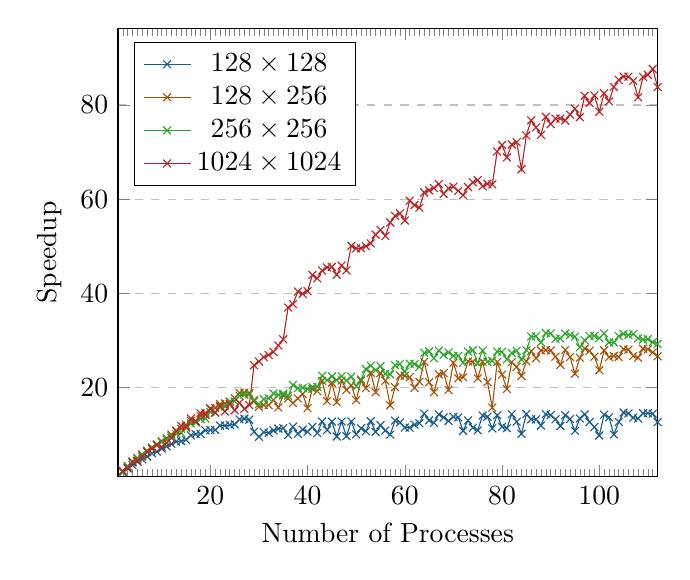
\begin{tikzpicture}
      \begin{axis}[
        xlabel={Number of Processes},
        ylabel={Speedup},
        xmin = 1, xmax = 112,
        ymin = 1,
        % xtick={0, 5, 10, 15, 20, 25},
        % ytick={0,20,40,60,80,100,120},
        legend pos=north west,
        ymajorgrids=true,
        grid style=dashed,
        minor xtick = {1, 2, 3, 4, 5, 6, 7, 8, 9, 10, 11, 12, 13, 14, 15, 16, 17, 18, 19, 20, 21, 22, 23, 24, 25, 26, 27, 28, 29, 30, 31, 32, 33, 34, 35, 36, 37, 38, 39, 40, 41, 42, 43, 44, 45, 46, 47, 48, 49, 50, 51, 52, 53, 54, 55, 56, 57, 58, 59, 60, 61, 62, 63, 64, 65, 66, 67, 68, 69, 70, 71, 72, 73, 74, 75, 76, 77, 78, 79, 80, 81, 82, 83, 84, 85, 86, 87, 88, 89, 90, 91, 92, 93, 94, 95, 96, 97, 98, 99, 100, 101, 102, 103, 104, 105, 106, 107, 108, 109, 110, 111, 112}
      ]
      \addlegendentry{$128\times128$}
      \addplot[color = {rgb:red,31;green,119;blue,180}, mark = x]coordinates{
        (1)
        (2, 1.923484904)
        (3, 2.720894881)
        (4, 3.440629879)
        (5, 4.138267014)
        (6, 4.663357796)
        (7, 5.242110909)
        (8, 5.997834661)
        (9, 6.289791841)
        (10, 6.946565607)
        (11, 7.428037519)
        (12, 7.95038628)
        (13, 8.433876381)
        (14, 8.529248058)
        (15, 8.803834029)
        (16, 9.766209845)
        (17, 10.03121078)
        (18, 10.06840901)
        (19, 10.823501)
        (20, 10.89601518)
        (21, 10.91800443)
        (22, 11.84262736)
        (23, 11.8219416)
        (24, 11.97369741)
        (25, 12.0975617)
        (26, 13.1584053)
        (27, 13.31030358)
        (28, 13.09199604)
        (29, 10.51279543)
        (30, 9.447423254)
        (31, 10.42385535)
        (32, 10.30054902)
        (33, 10.80235067)
        (34, 11.18228843)
        (35, 11.28177199)
        (36, 9.84586148)
        (37, 11.58823901)
        (38, 10.08001059)
        (39, 10.99390174)
        (40, 10.5569982)
        (41, 11.56726497)
        (42, 10.24545739)
        (43, 12.72036597)
        (44, 10.89204809)
        (45, 12.68270324)
        (46, 9.517212061)
        (47, 12.70287876)
        (48, 9.582852227)
        (49, 12.70536401)
        (50, 9.965823544)
        (51, 11.25846097)
        (52, 10.63104034)
        (53, 12.76248403)
        (54, 10.50652785)
        (55, 11.90630364)
        (56, 10.76817156)
        (57, 9.92607211)
        (58, 12.89249626)
        (59, 12.51463609)
        (60, 11.41730712)
        (61, 11.38075986)
        (62, 12.05183804)
        (63, 12.33484451)
        (64, 14.36825721)
        (65, 12.94409609)
        (66, 12.41719085)
        (67, 14.19480666)
        (68, 13.57486626)
        (69, 12.82320169)
        (70, 13.70570713)
        (71, 13.56967231)
        (72, 10.71067935)
        (73, 12.95178741)
        (74, 11.37959467)
        (75, 10.82015609)
        (76, 13.97900377)
        (77, 13.7270023)
        (78, 11.23829384)
        (79, 14.05923951)
        (80, 11.55316639)
        (81, 11.2926889)
        (82, 14.27943961)
        (83, 12.66856962)
        (84, 10.09500034)
        (85, 14.28261536)
        (86, 13.16863695)
        (87, 13.18328092)
        (88, 11.84068965)
        (89, 14.27750429)
        (90, 14.05330958)
        (91, 13.16981575)
        (92, 11.72223637)
        (93, 14.04375416)
        (94, 13.24823774)
        (95, 10.70439261)
        (96, 13.35667621)
        (97, 14.2305021)
        (98, 12.59951023)
        (99, 11.54477978)
        (100, 9.726436232)
        (101, 14.16020099)
        (102, 13.58441421)
        (103, 9.940775763)
        (104, 12.61740837)
        (105, 14.60476445)
        (106, 14.41749489)
        (107, 13.5330826)
        (108, 13.33602024)
        (109, 14.45781616)
        (110, 14.46196727)
        (111, 14.37893291)
        (112, 12.55231676)
      };
      \addlegendentry{$128\times256$}
      \addplot[color = {rgb:red,255;green,127;blue,14}, mark = x]coordinates{
        (1)
        (2, 2.205625975)
        (3, 3.227329026)
        (4, 4.206536128)
        (5, 4.957628857)
        (6, 5.720325252)
        (7, 6.5186293)
        (8, 7.204187632)
        (9, 7.83187371)
        (10, 8.519480837)
        (11, 9.141792188)
        (12, 9.946144856)
        (13, 10.78303952)
        (14, 11.17654785)
        (15, 11.96372797)
        (16, 12.86100085)
        (17, 12.77900855)
        (18, 13.84474552)
        (19, 14.54722804)
        (20, 15.51467595)
        (21, 15.61471426)
        (22, 16.41110324)
        (23, 16.55474236)
        (24, 16.88471919)
        (25, 17.63506903)
        (26, 18.81278116)
        (27, 18.85990554)
        (28, 18.79353144)
        (29, 16.99774639)
        (30, 15.79817866)
        (31, 16.19702524)
        (32, 16.15965593)
        (33, 17.29162535)
        (34, 15.70016114)
        (35, 18.24326824)
        (36, 17.59400273)
        (37, 16.60271485)
        (38, 17.62056876)
        (39, 18.54799616)
        (40, 15.55440163)
        (41, 19.67959722)
        (42, 19.1560423)
        (43, 21.35522276)
        (44, 17.03686616)
        (45, 20.92098931)
        (46, 16.81730667)
        (47, 21.42591543)
        (48, 19.41596955)
        (49, 20.40834137)
        (50, 17.25017866)
        (51, 21.42281112)
        (52, 19.78933109)
        (53, 23.07737542)
        (54, 18.918754)
        (55, 23.01384332)
        (56, 21.37017128)
        (57, 16.14969542)
        (58, 20.0009934)
        (59, 22.46020712)
        (60, 22.42917414)
        (61, 22.12510191)
        (62, 19.87277518)
        (63, 21.15162638)
        (64, 25.37114287)
        (65, 21.04839449)
        (66, 18.95802252)
        (67, 22.70932312)
        (68, 22.97178595)
        (69, 19.42403684)
        (70, 25.20246959)
        (71, 21.87162616)
        (72, 22.10931871)
        (73, 25.48457214)
        (74, 25.40576875)
        (75, 21.86621052)
        (76, 25.42855553)
        (77, 21.08392509)
        (78, 15.6640675)
        (79, 25.37761189)
        (80, 22.68812171)
        (81, 19.62011193)
        (82, 25.34038719)
        (83, 24.32976857)
        (84, 22.38365252)
        (85, 25.49728852)
        (86, 27.67149109)
        (87, 26.16157312)
        (88, 27.82572378)
        (89, 27.90751086)
        (90, 27.82654636)
        (91, 26.48489496)
        (92, 24.75372864)
        (93, 27.9508939)
        (94, 26.41014954)
        (95, 22.85484751)
        (96, 26.26628274)
        (97, 28.21556741)
        (98, 27.73270133)
        (99, 26.49618844)
        (100, 23.61317402)
        (101, 27.82729043)
        (102, 26.40723599)
        (103, 26.65524278)
        (104, 26.4087459)
        (105, 28.08446357)
        (106, 27.97894075)
        (107, 26.65102998)
        (108, 26.26789063)
        (109, 28.17805085)
        (110, 28.07259611)
        (111, 27.39171519)
        (112, 26.56061497)
      };
      \addlegendentry{$256\times256$}
      \addplot[color = {rgb:red,44;green,160;blue,44}, mark = x]coordinates{
        (1)
        (2, 1.925127415)
        (3, 3.140333019)
        (4, 4.034925801)
        (5, 4.78762859)
        (6, 5.548938663)
        (7, 6.404618662)
        (8, 6.968739974)
        (9, 7.663080488)
        (10, 8.312526115)
        (11, 8.852461517)
        (12, 9.605431059)
        (13, 10.06145238)
        (14, 10.29374937)
        (15, 11.37306684)
        (16, 12.28185633)
        (17, 12.50338781)
        (18, 13.18889042)
        (19, 13.31294585)
        (20, 14.70777733)
        (21, 14.55264271)
        (22, 15.75611214)
        (23, 15.92868238)
        (24, 16.95789156)
        (25, 17.02232096)
        (26, 18.1996368)
        (27, 18.42801124)
        (28, 18.46672465)
        (29, 17.29202644)
        (30, 16.3773773)
        (31, 17.47308485)
        (32, 17.62638401)
        (33, 18.65075869)
        (34, 18.39755995)
        (35, 18.60686115)
        (36, 18.19979983)
        (37, 20.47095888)
        (38, 19.78039772)
        (39, 19.87870191)
        (40, 19.57366035)
        (41, 20.0423534)
        (42, 20.04684952)
        (43, 22.41860194)
        (44, 21.51447621)
        (45, 22.29960449)
        (46, 21.51985585)
        (47, 22.32706386)
        (48, 21.42352302)
        (49, 22.23288533)
        (50, 20.21625868)
        (51, 21.66294914)
        (52, 23.84329098)
        (53, 24.58609618)
        (54, 23.59494944)
        (55, 24.47228876)
        (56, 22.8398099)
        (57, 22.7149941)
        (58, 24.69497187)
        (59, 24.92866935)
        (60, 23.2764513)
        (61, 25.00215927)
        (62, 24.92609823)
        (63, 24.28449993)
        (64, 27.31102246)
        (65, 27.61766033)
        (66, 26.16929081)
        (67, 27.76095551)
        (68, 26.85523603)
        (69, 27.40893503)
        (70, 26.66846158)
        (71, 26.67769083)
        (72, 25.19788674)
        (73, 27.57875103)
        (74, 27.87808785)
        (75, 25.09623612)
        (76, 27.80856085)
        (77, 25.41232735)
        (78, 25.61260696)
        (79, 27.60106957)
        (80, 27.50554548)
        (81, 25.9284344)
        (82, 27.30692535)
        (83, 27.73519686)
        (84, 25.88250583)
        (85, 27.85795858)
        (86, 30.78228538)
        (87, 30.86531039)
        (88, 29.51948872)
        (89, 31.51723922)
        (90, 31.42733336)
        (91, 30.28669265)
        (92, 30.36085084)
        (93, 31.41414203)
        (94, 31.09725455)
        (95, 30.76079515)
        (96, 28.47261565)
        (97, 29.97695709)
        (98, 30.87137952)
        (99, 30.90962268)
        (100, 30.42258674)
        (101, 31.43276204)
        (102, 29.50436935)
        (103, 29.53203012)
        (104, 30.86278203)
        (105, 31.34884069)
        (106, 31.08695855)
        (107, 31.28857046)
        (108, 30.40892566)
        (109, 30.13636152)
        (110, 30.2196501)
        (111, 29.55258643)
        (112, 29.19595139)
      };
      \addlegendentry{$1024\times1024$}
      \addplot[color = {rgb:red,214;green,39;blue,40}, mark = x]coordinates{
        (1)
        (2, 2.173711193)
        (3, 2.836895868)
        (4, 4.036873172)
        (5, 4.389001279)
        (6, 5.250171877)
        (7, 6.206328606)
        (8, 6.884988543)
        (9, 7.699455735)
        (10, 7.326102008)
        (11, 8.167957305)
        (12, 9.202796572)
        (13, 10.64605845)
        (14, 11.79316736)
        (15, 11.54612272)
        (16, 13.36192713)
        (17, 12.76637316)
        (18, 14.4268392)
        (19, 14.09500759)
        (20, 15.37438851)
        (21, 14.63591628)
        (22, 15.99456741)
        (23, 14.83351358)
        (24, 16.4555638)
        (25, 15.07849263)
        (26, 16.68441375)
        (27, 15.42876319)
        (28, 16.17670295)
        (29, 24.68537945)
        (30, 25.46714682)
        (31, 26.39691444)
        (32, 26.8356459)
        (33, 27.49939443)
        (34, 28.87062298)
        (35, 30.18922927)
        (36, 36.93424484)
        (37, 37.6672039)
        (38, 40.34303667)
        (39, 39.8556408)
        (40, 40.41454983)
        (41, 43.87475629)
        (42, 43.1394357)
        (43, 44.8060583)
        (44, 45.47120956)
        (45, 45.5843428)
        (46, 43.9177163)
        (47, 45.85590864)
        (48, 44.81901113)
        (49, 50.05752876)
        (50, 49.50540648)
        (51, 49.54762095)
        (52, 49.96750344)
        (53, 50.58992914)
        (54, 52.44384123)
        (55, 53.4581716)
        (56, 52.14910419)
        (57, 55.02558376)
        (58, 56.41919087)
        (59, 56.94366787)
        (60, 55.43683673)
        (61, 59.66312456)
        (62, 58.74375724)
        (63, 58.16551375)
        (64, 61.3999277)
        (65, 61.85867302)
        (66, 62.34991401)
        (67, 63.19022701)
        (68, 61.10059992)
        (69, 62.28022212)
        (70, 62.6293099)
        (71, 61.73663883)
        (72, 60.82668503)
        (73, 62.5723675)
        (74, 63.56593066)
        (75, 64.00574238)
        (76, 62.73501572)
        (77, 63.27787491)
        (78, 63.1338179)
        (79, 70.12503895)
        (80, 71.49919016)
        (81, 68.86425241)
        (82, 71.60464349)
        (83, 72.09983165)
        (84, 66.33512191)
        (85, 73.53397362)
        (86, 76.75693789)
        (87, 75.24787807)
        (88, 73.65530039)
        (89, 77.50192905)
        (90, 75.94842153)
        (91, 77.12477113)
        (92, 77.12126478)
        (93, 76.71422997)
        (94, 77.95088847)
        (95, 79.2228139)
        (96, 77.41345895)
        (97, 81.95770308)
        (98, 80.44184872)
        (99, 82.03430774)
        (100, 78.57669283)
        (101, 82.48412344)
        (102, 80.78814024)
        (103, 83.86361613)
        (104, 85.34170442)
        (105, 86.05367642)
        (106, 86.03765818)
        (107, 85.12883448)
        (108, 81.64434285)
        (109, 85.96417874)
        (110, 86.41459805)
        (111, 87.66408809)
        (112, 83.83735179)
      };
      \end{axis}
    \end{tikzpicture}
  }
  \caption{Speedup curves for my MPI implementation}\label{fig:scaling}
\end{figure}

My implementation initially scaled well for the smallest three grid sizes, but the speedup acquired from each subsequent process declined (i.e. a sublinear plateau), which occurred due to several reasons.
Firstly, perfect linear scaling was theoretically impossible because the program contained serial sections.

My implementation followed a similar pattern for the $1024 \times 1024$ grid, however there was a clear increase in speedup after approximately 30 processes.
The superlinear speedup at this point was caused by the largest problem size being split sufficiently small to fit into the L3 cache.

\subsection{Comparison to Serial}

\section{Hybrid MPI and OpenMP}

I sought to investigate whether a hybrid implementation would execute faster than my prior implementation.

\subsection{OpenMP vs MPI Scaling}

Before producing my hybrid implementation, I compared the speedup curves of my distributed memory parallelism implementation built with MPI with my shared-memory parallelism implementation built with OpenMP.
Figure \ref{fig:scaling_openmp_mpi} displays the speedup curves of these two implementations with the $128 \times 128$ and the $1024 \times 1024$ grid sizes.

\begin{figure}[htpb]
  \centering
  \resizebox{\columnwidth}{!}{
    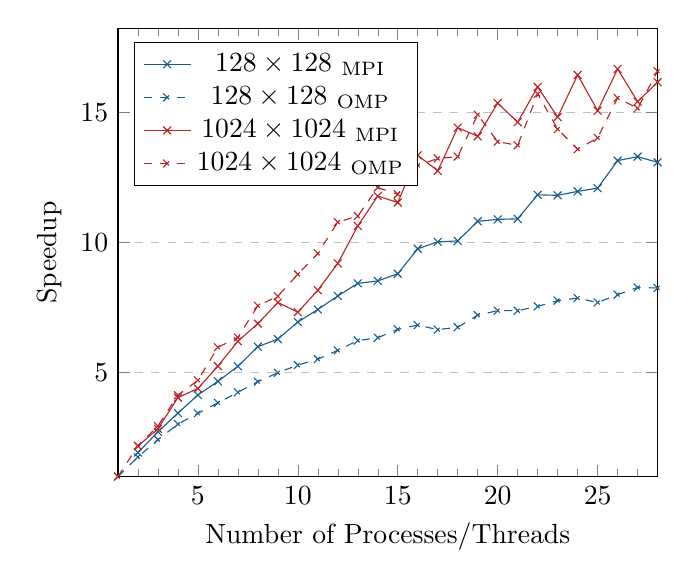
\begin{tikzpicture}
      \begin{axis}[
        xlabel={Number of Processes/Threads},
        ylabel={Speedup},
        xmin = 1, xmax = 28,
        ymin = 1,
        % xtick={0, 5, 10, 15, 20, 25},
        % ytick={0,20,40,60,80,100,120},
        legend pos=north west,
        ymajorgrids=true,
        grid style=dashed,
        minor xtick = {1, 2, 3, 4, 5, 6, 7, 8, 9, 10, 11, 12, 13, 14, 15, 16, 17, 18, 19, 20, 21, 22, 23, 24, 25, 26, 27, 28}
      ]
      \addlegendentry{$128\times128$ \textsubscript{MPI}}
      \addplot[color = {rgb:red,31;green,119;blue,180}, mark = x]coordinates{
        (1)
        (2, 1.923484904)
        (3, 2.720894881)
        (4, 3.440629879)
        (5, 4.138267014)
        (6, 4.663357796)
        (7, 5.242110909)
        (8, 5.997834661)
        (9, 6.289791841)
        (10, 6.946565607)
        (11, 7.428037519)
        (12, 7.95038628)
        (13, 8.433876381)
        (14, 8.529248058)
        (15, 8.803834029)
        (16, 9.766209845)
        (17, 10.03121078)
        (18, 10.06840901)
        (19, 10.823501)
        (20, 10.89601518)
        (21, 10.91800443)
        (22, 11.84262736)
        (23, 11.8219416)
        (24, 11.97369741)
        (25, 12.0975617)
        (26, 13.1584053)
        (27, 13.31030358)
        (28, 13.09199604)
      };
      \addlegendentry{$128\times128$ \textsubscript{OMP}}
      \addplot[color = {rgb:red,31;green,119;blue,180}, mark = x, dashed]coordinates{
        (1, 1.0)
        (2, 1.7525169788462858)
        (3, 2.419897249840069)
        (4, 3.0177321760395954)
        (5, 3.4340474353625594)
        (6, 3.8362657949346852)
        (7, 4.241072726461517)
        (8, 4.651864978037027)
        (9, 4.993654422331282)
        (10,5.2882280154084835)
        (11,5.520195387872089)
        (12,5.854579031493787)
        (13,6.23457059163917)
        (14,6.342501046595846)
        (15,6.666023078680611)
        (16,6.829810732132427)
        (17,6.6526516481296065)
        (18,6.746204776109836)
        (19,7.213003419569139)
        (20,7.383978810814603)
        (21,7.383266518002555)
        (22,7.548589923892521)
        (23,7.770076587082373)
        (24,7.86829502746941)
        (25,7.69660960948019)
        (26,8.000150678051229)
        (27,8.274732001825265)
        (28,8.256913368882064)
      };
      \addlegendentry{$1024\times1024$ \textsubscript{MPI}}
      \addplot[color = {rgb:red,214;green,39;blue,40}, mark = x]coordinates{
        (1)
        (2, 2.173711193)
        (3, 2.836895868)
        (4, 4.036873172)
        (5, 4.389001279)
        (6, 5.250171877)
        (7, 6.206328606)
        (8, 6.884988543)
        (9, 7.699455735)
        (10, 7.326102008)
        (11, 8.167957305)
        (12, 9.202796572)
        (13, 10.64605845)
        (14, 11.79316736)
        (15, 11.54612272)
        (16, 13.36192713)
        (17, 12.76637316)
        (18, 14.4268392)
        (19, 14.09500759)
        (20, 15.37438851)
        (21, 14.63591628)
        (22, 15.99456741)
        (23, 14.83351358)
        (24, 16.4555638)
        (25, 15.07849263)
        (26, 16.68441375)
        (27, 15.42876319)
        (28, 16.17670295)
      };
      \addlegendentry{$1024\times1024$ \textsubscript{OMP}}
      \addplot[color = {rgb:red,214;green,39;blue,40}, mark = x, dashed]coordinates{
        (1, 1)
        (2, 2.182054561)
        (3, 2.943754524)
        (4, 4.131667716)
        (5, 4.705750019)
        (6, 5.973656817)
        (7, 6.351981192)
        (8, 7.573833461)
        (9, 7.941396106)
        (10,8.7813412)
        (11,9.58468842)
        (12,10.78916878)
        (13,11.02458512)
        (14,12.12324785)
        (15,11.86351157)
        (16,12.97218687)
        (17,13.23885542)
        (18,13.31481491)
        (19,14.92644603)
        (20,13.88484436)
        (21,13.74639988)
        (22,15.72695273)
        (23,14.36825215)
        (24,13.59839996)
        (25,14.03417467)
        (26,15.5747082)
        (27,15.16956075)
        (28,16.59876059)
      };
      \end{axis}
    \end{tikzpicture}
  }
  \caption{Speedup curves for my OpenMP and MPI implementation}\label{fig:scaling_openmp_mpi}
\end{figure}

My MPI implementation scaled better for the smaller grid, whereas my OpenMP implementation initially scaled slightly better for the larger grid.
This was because each implementation had a different overhead: in the OpenMP implementation, the overhead arose from the creation and synchronisation of threads each timestep; in the MPI implementation, the overhead arose from the halo exchange.
The OpenMP overhead was largely constant regardless of the grid size, whereas the MPI overhead was correlated with the width of the grid.

\subsection{Implementation}

Having gained an understanding of how my OpenMP and MPI implementations scaled, I hypothesised that a hybrid implementations would reduce the execution times for large, wide grid sizes.
Therefore, I produced three additional grids to test my implementation with.

Using my prior implementation as a starting point, I replaced the call to the \texttt{MPI\_Init} procedure with a call to the \texttt{MPI\_Init\_thread} procedure, passing \texttt{MPI\_THREAD\_FUNNELED} as the third argument since only the main thread was to make MPI calls.
I parallelised the outer loop in the \texttt{timestep} procedure with OpenMP, and set the \texttt{I\_MPI\_PIN\_DOMAIN} environment variable to \texttt{socket}.

I tested my implementation with eight processes---one per socket across four nodes---communicating via MPI, with each process creating fourteen threads.
Table \ref{tab:hybrid} displays the results of my experiment.
As anticipated, the hybrid implementation was slower with the smaller grids that were provided, but faster with the larger grids that I produced myself.

\begin{table}[htbp]
  \begin{center}
  \caption{Execution times with the hybrid implementation and speedup over the prior implementation}\label{tab:hybrid}
  \begin{tabular}[t]{l | l l} 
      \hline\hline
      Grid Size&Time (s)&Speedup\\
      \hline
      $128 \times 128$&\texttt{ \space0.67}&\texttt{}\\
      $128 \times 256$&\texttt{ \space0.73}&\texttt{}\\
      $256 \times 256$&\texttt{ \space1.94}&\texttt{}\\
      $1024 \times 1024$&\texttt{ \space3.17}&\texttt{}\\
      \hdashline
      $4096 \times 1024$&\texttt{ 15.99}&\texttt{1.42}\\
      $8192 \times 1024$&\texttt{ 53.88}&\texttt{1.03}\\
      $16384 \times 1024$&\texttt{102.34}&\texttt{1.15}\\
      \hline
    \end{tabular}
  \end{center}
\end{table}

\section{GPU Programming}

GPUs typically have 3--5x the memory bandwidth, and 5--10x the peak FLOP/s that CPUs have.
This is true for BC4, in which a single NVIDIA Tesla P100 has 4.8x the peak memory bandwidth, and 9.8x the peak double precision performance than two Intel E5-2840 v4 CPUs have.
OpenCL is a framework for heterogeneous computing that can be used for GPU programming.
I sought to produce an implementation of LBM to run on a single NVIDIA Tesla P100 to identify how fast it could run.

\subsection{Implementation}

I used my serial optimised implementation as a starting point for my host program.
To ensure my program was portable, I used the \texttt{clGetPlatformIDs} and \texttt{clGetDeviceIDs} procedures to produce an array of all devices available to the host program, and selected the device defined by the \texttt{OCL\_DEVICE} environment variable.
For the selected device, I created a single context and a single in-order queue.
I opted to keep my \texttt{cells} and \texttt{cells\_new} data in the SoA format, since coalesced memory accesses are key for high bandwidth.

I converted the \texttt{accelerate\_flow} and \texttt{timestep} procedures into kernels to run on the GPU.
Transerring memory between host and device is a slow operation; therefore, I opted to store the partial average velocities of each timestep in global memory on the device.
Each timestep, the \texttt{timestep} kernel performed a parallel reduction to sum the average velocities of each cell in the same work group.
I opted to implement a parallel reduction to prevent a single item in the work group 


Parallel reduction.

\begin{table}[htbp]
  \begin{center}
  \caption{Execution times with the OpenCL implementation and speedup over the serial implementation}\label{tab:OpenCL_1}
  \begin{tabular}[t]{l | l l} 
      \hline\hline
      Grid Size&Time (s)&Speedup\\
      \hline
      $128 \times 128$&\texttt{}&\texttt{}\\
      $128 \times 256$&\texttt{}&\texttt{}\\
      $256 \times 256$&\texttt{}&\texttt{}\\
      $1024 \times 1024$&\texttt{}&\texttt{}\\
      \hdashline
      $2048 \times 2048$&\texttt{}&\texttt{}\\
      $4096 \times 4096$&\texttt{}&\texttt{}\\
      \hline
    \end{tabular}
  \end{center}
\end{table}

\subsection{Work-Group Size}

\begin{table}[htbp]
  \begin{center}
  \caption{Execution times with the OpenCL implementation and speedup over the prior implementation}\label{tab:OpenCL_2}
  \begin{tabular}[t]{l | l l} 
      \hline\hline
      Grid Size&Time (s)&Speedup\\
      \hline
      $128 \times 128$&\texttt{}&\texttt{}\\
      $128 \times 256$&\texttt{}&\texttt{}\\
      $256 \times 256$&\texttt{}&\texttt{}\\
      $1024 \times 1024$&\texttt{}&\texttt{}\\
      \hline
    \end{tabular}
  \end{center}
\end{table}

\section{Conclusion}

\printbibliography

\end{document}